\chapter{\label{d}Signal and Background}
What are signal and background? The signal corresponds to the features, process, or whatever events we are interested in studying. This signal could correspond to the production of a Higgs, or maybe of a pair of W bosons, or maybe it just corresponds to events with two high energy jets or events in them. While the backgrounds are the events that may seem like signals but we are not interested in.\\
We took s simulated sample of the resonance particles of the top quark; Tprime, and other t-quark particle such as $\Bar{t}tH$, thq, and ttgg for the training and testing of the deep neural network model.
The associated production of top quarks with the Higgs boson, either in pairs ($\Bar{t}tH$) or singly (tH), provides direct experimental access to the top-Higgs
coupling. The $\Bar{t}tH (tH)$ production mode, while proceeding at a rate of about 100(1000) times smaller than gluon fusion, bears a highly distinctive experimental signature, which includes leptons and/or jets from the decay of the two (single) top quarks as shown in \autoref{fig:my_label_tth}. \\
With the increase of the LHC energy from 8 to 13 TeV for Run 2, the ttH production cross section is expected to increase by a factor four. However, such process still remains rare, and searches for ttH production have been driven by the higher sensitivity achieved in Higgs decay modes with larger branching fractions.[\cite{14}] \\
\begin{figure}[H]
    \centering
    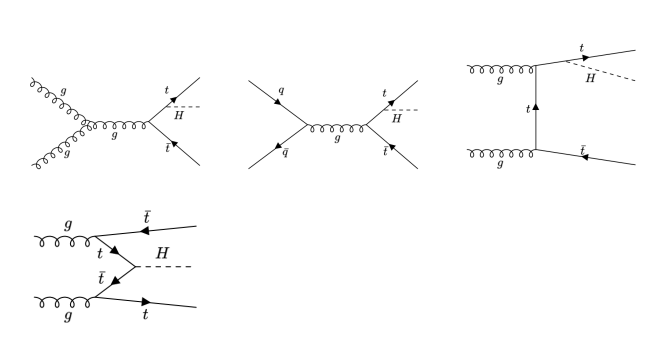
\includegraphics[scale=0.7]{tth_1.png}
    \caption{Feynman diagrams depicting $t\Bar{t}H$ production modes}
    \label{fig:my_label_tth}
\end{figure}


As the standard model(SM) is complete as a low-energy effective theory describing all known fundamental particles and their interactions. But there are also a few problems that SM cannot explain. There are various theories of new physics beyond the SM that predict the additional particles that can affect the quantum corrections to the Higgs boson mass and answer question, which is known as "hierarchy problem". One of the proposed promising new states is vector-like quarks.\cite{12}

Vector-like quarks (VLQs) are hypothetical spin-1/2 coloured particles, labeled $T^'$ and $B’$, with electric charges of +2e/3 and -1e/3, respectively. Their left-handed and right-handed components transform in the same way under the Standard Model gauge group. A vector-like top quark partner T' has two production modes. One is pair production through the strong interaction while the other is single production mode through the electroweak interaction\cite{12}. The T' quark could couple to bW, tZ, or tH, resulting in the corresponding T' quark decays as shown with Feynman diagram in the \autoref{fig:my_label_T'}. We will use this VLQ as the signal.\\




\begin{figure}[H]
    \centering
    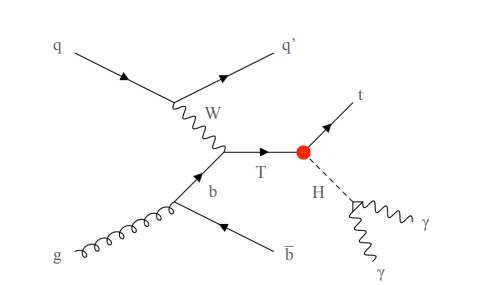
\includegraphics[scale=0.5]{T'.png}
    \caption{Leading-order Feynman diagram for single T’ production}
    \label{fig:my_label_T'}
\end{figure}





For the another two ntuples of thq and ttgg, the Feynman diagrams are plotted in the  \autoref{fig:my_label_ttgg}, \autoref{fig:my_label_ttgg_12}, and \autoref{fig:my_label_thq}  respectively.

\begin{figure}[H]
    \centering
    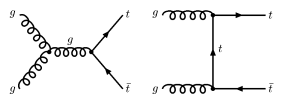
\includegraphics[scale=0.5]{ttgg.png}
    \caption{ttgg Feynman diagram}
    \label{fig:my_label_ttgg}
\end{figure}

\begin{figure}[H]
    \centering
    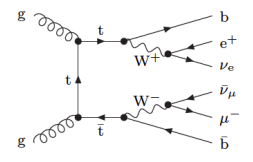
\includegraphics[scale=0.5]{ttgg__.png}
    \caption{Feynman diagram for ttgg}
    \label{fig:my_label_ttgg_12}
\end{figure}




\begin{figure}[H]
    \centering
    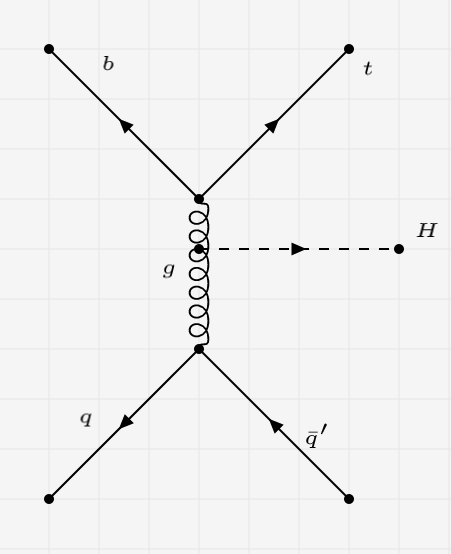
\includegraphics[scale =0.5]{thq.png}
    \caption{Feynman diagram of thq}
    \label{fig:my_label_thq}
\end{figure}




Few of the plots of variables of these simulated samples are shown below,
\begin{figure}[H]
\begin{subfigure}{.5\textwidth}
  \centering
  % include first image
  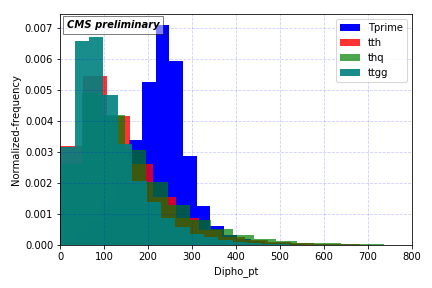
\includegraphics[width=.8\linewidth]{Inputs/variable_Dipho_pt.png}  
  \caption{}
  \label{fig:sub-first}
\end{subfigure}
\begin{subfigure}{.5\textwidth}
  \centering
  % include second image
  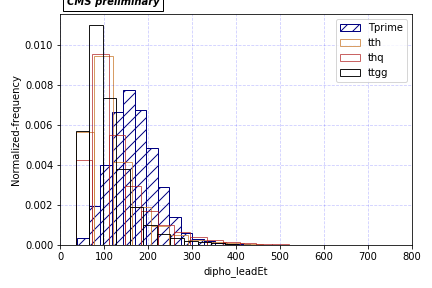
\includegraphics[width=.8\linewidth]{Inputs/variable_Dipho_leadEta.png}  
  \caption{}
  \label{fig:sub-second}
\end{subfigure}



\begin{subfigure}{.5\textwidth}
  \centering
  % include third image
  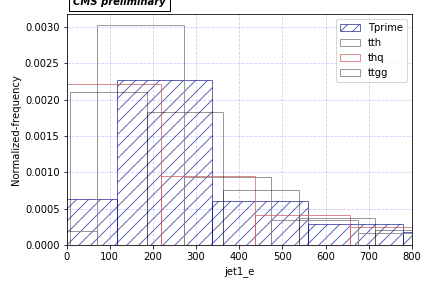
\includegraphics[width=.8\linewidth]{Inputs/variable_jet1_e.png}  
  \caption{}
  \label{fig:sub-third}
\end{subfigure}
\begin{subfigure}{.5\textwidth}
  \centering
  % include fourth image
  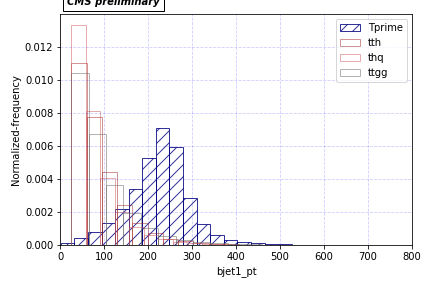
\includegraphics[width=.8\linewidth]{Inputs/variable_bjet1_pt.png}  
  \caption{}
  \label{fig:sub-fourth}
\end{subfigure}


\begin{subfigure}{.5\textwidth}
  \centering
  % include third image
  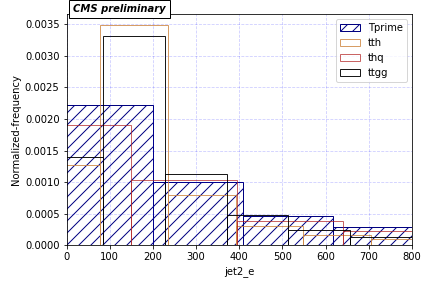
\includegraphics[width=.8\linewidth]{Inputs/jet2_e.png}  
  \caption{}
  \label{fig:sub-fifth}
\end{subfigure}
\begin{subfigure}{.5\textwidth}
  \centering
  % include fourth image
  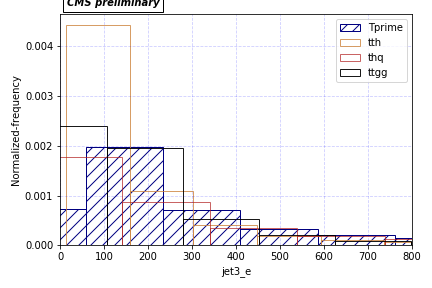
\includegraphics[width=.8\linewidth]{Inputs/jet3_e.png}  
  \caption{}
  \label{fig:sub-fourth}
\end{subfigure}

\begin{subfigure}{.5\textwidth}
  \centering
  % include third image
  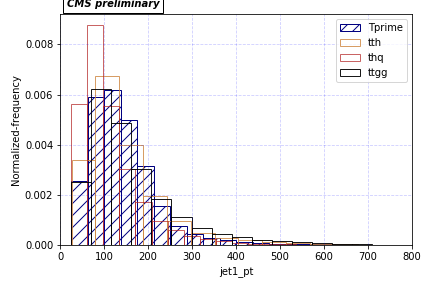
\includegraphics[width=.8\linewidth]{Inputs/jet1_pt.png}  
  \caption{}
  \label{fig:sub-third}
\end{subfigure}
% \begin{subfigure}{.5\textwidth}
%   \centering
%   % include fourth image
%   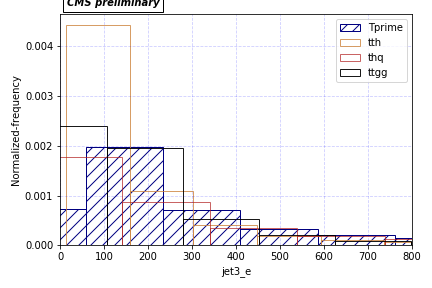
\includegraphics[width=.8\linewidth]{Inputs/jet3_e.png}  
%   \caption{}
%   \label{fig:sub-fourth}
% \end{subfigure}
\caption{Simulated sample plot for different variables, for each figure plotted above the signal is Tprime and the background is tth, thq, and ttgg. From top to bottom, plots for different variable are as, (a) Plot for $Dipho\_P_T$, (b) Plot for $Dipho\_leadEt$, (c)Plot for $jet1\_e$, (d) Plot for $bjet1\_P_T$, (e) Plot for $jet2\_e$, (f) Plot for $jet3\_e$, and (g) Plot for $jet1\_P_T$ }
\label{fig:fig}
\end{figure}
 
In the given \autoref{fig:fig}, we plotted a representation for a few variables. from this figure, we can see how our signal (Tprime) cannot get clearly separated from our background( $tt\gamma \gamma$, $\Bar{t}th$, and thq. Our main motivation is to make a better separation of the Tprime, signal in this case from the backgrounds i.e., $tt\gamma\gamma$, $\Bar{t}th$, and thq.








% Questions needed to be addressed?
% \begin{itemize}
%     \item What are signal and background?
%     \item 
% \end{itemize}































% About Simulated sample 
%     \begin{itemize}
    
%         % \item Feynman Diagram(details about tth, ttgg, thq, Tprime)
%         \item Kinematics features, Kinematic variables definition and its derivations(about all of the variables and their meaning)
%         \item 
%         \item What feature of (suppose $Dipho_PT$) you are measuring.
%         % \item What is Tprime, tth, thq, ttgg? How these are formed
%         % \item how the varibale looks lie. Present a few of them
        
%     \end{itemize}
    
    

\setcounter{equation}{0}
\setcounter{table}{0}
\setcounter{figure}{0}
%\baselineskip 24pt


% %%%%%%%%%%%%%%%%%%%%%%QUESTIONS MAY GET FRAMED FROM HERE%%%%%%%%%%%%%%%%%%%%%%%%%%%%%%%%%%%%%%%%%%%%%%
% \begin{itemize}
%     \item Why we measure luminosity in $fb^{-1}$
% \end{itemize}